\section{Experiments}

Experiments are done with two agent based models in three regions with different population sizes. Number of agents in each of the region are as follows: Rappahannock county has 2495 agents, San Diego has 12925 agents, Shenandoah Valley Region (SVR) has 138043 agents. 

\begin{figure}
    \centering
    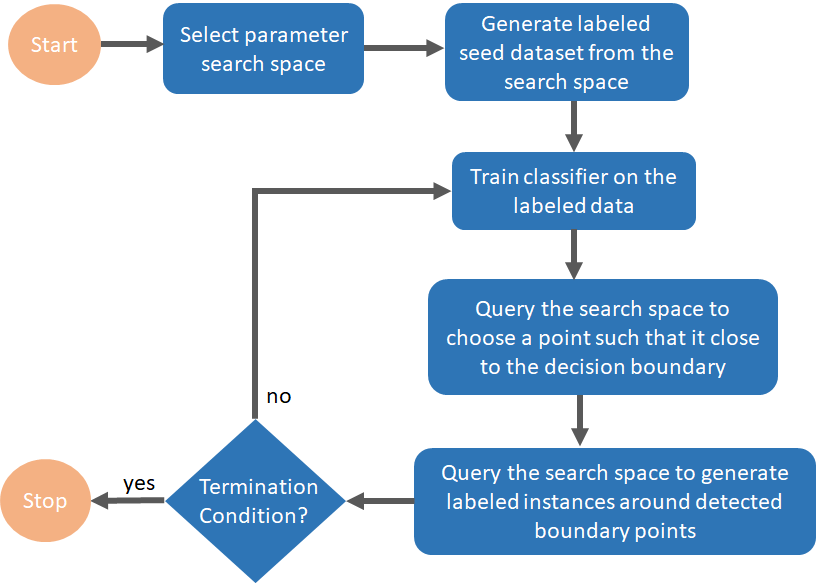
\includegraphics{AAMAS20Template-submission/figures/workflow.png}
    \caption{Overview of the presented methodology - A common set of parameters is chosen from both ABMs and an active learning framework is implemented to learn the decision boundary that separates small and large solar panel adoptions. }
    \label{fig:workflow}
\end{figure}

Both the agent-based diffusion models simulate the number of households adopting rooftop solar.
The model presented in Section \ref{virginia_model} is used for Rappahannock county in Virginia and Shenandoah Valley Region in Virginia. 
The model presented in Section \ref{san-diego-model} is used for San Diego.
In order to facilitate comparison between the 2 ABMs, we choose to explore the common parameters in both the models: Mile1 and NPV. All experiments are conducted in 2D space using Mile1 and NPV.

Before learning the decision boundary that separates the low and high adoptions for the three regions, we need to set the parameter extents of the search space, $STDEV-THRESHOLD$ for boundary point condition, and $MEAN-THRESHOLD$ for labeling points evaluated in the search space. Diffusion model outputs are examined for points across the diagonal of an arbitrary parameter space. As an example, Figures \ref{fig:diagmean}, \ref{fig:diagstdev}, and \ref{fig:diagDisplay} show the output of the ABMs in terms of mean and standard deviation. On observing the sharp transitions in mean and standard deviation, $STDEV-THRESHOLD$ is set to 250 and $MEAN-THRESHOLD$ is set to 1000 for Rappahannock. Similar experiments are performed for SVR and San Diego regions to set the thresholds.
In all the experiment settings and results shown, the ABM results are averaged over 20 replicates to calculate mean and standard deviation. 
%If time out happens then we discard the point or process how many every replicates are completed.
{\color{magenta} Q for Samarth: Should we give the mean and stdev thresholds for each region?}

\begin{figure}
    \centering
    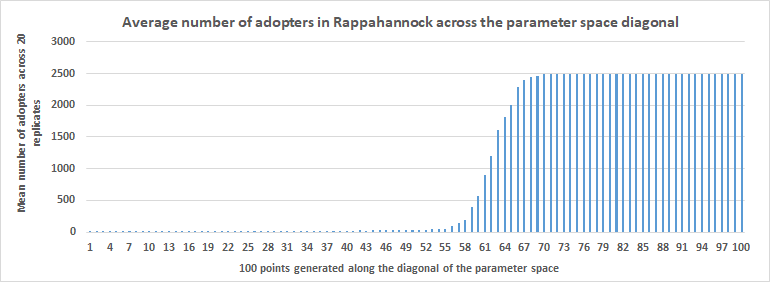
\includegraphics{AAMAS20Template-submission/figures/rapp-diag-mean1.png}
    \caption{Diagonal Mean <ADD MORE>}
    \label{fig:diagmean}
\end{figure}

\begin{figure}
    \centering
    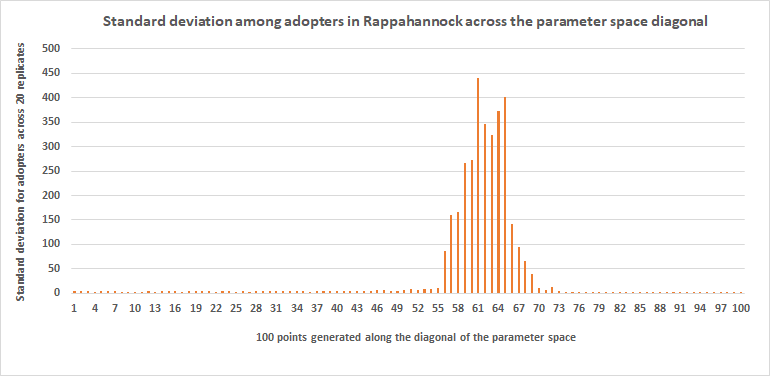
\includegraphics{AAMAS20Template-submission/figures/rapp-diag-stdev1.png}
    \caption{Diagonal Stdev <ADD MORE>}
    \label{fig:diagstdev}
\end{figure}

\begin{figure}
\begin{subfigure}{.25\textwidth}
  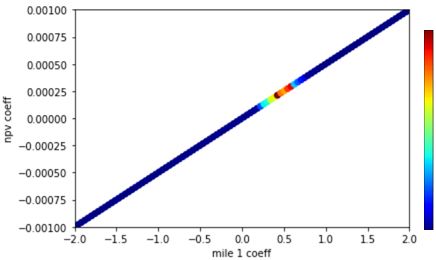
\includegraphics[height=3cm,width=4cm]{AAMAS20Template-submission/figures/rapp100diagstdev1.png}
    %\caption{Standard deviation for points on diagonal}
  %\label{fig:diagstdev}
\end{subfigure}%
\begin{subfigure}{.25\textwidth}
  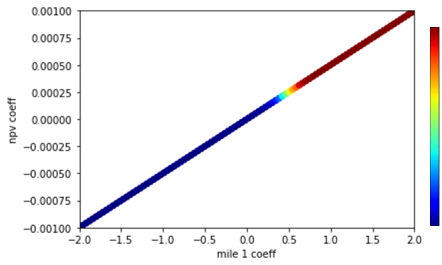
\includegraphics[height=3cm,width=4cm]{AAMAS20Template-submission/figures/rapp100diagmean1.png}
  %\caption{Mean for points on diagonal}
  %\label{fig:}
\end{subfigure}
\caption{Standard deviation and mean for points evaluated by ABM on the diagonal of the 2D search space. The colors blue to red represent transition from small outbreak to large outbreak. Some variability is observed for both mean and standard deviation between 0.3 to 0.6 on the x-axis which denotes the range for mile 1 coefficient. When seen in reference to Figure \ref{fig:diagRappMean} and Figure \ref{fig:diagRappStdev} this region shows a sharp transition from small outbreak to large outbreak.}
\label{fig:diagDisplay}
\end{figure}

\begin{comment}
\begin{figure}
    \centering
    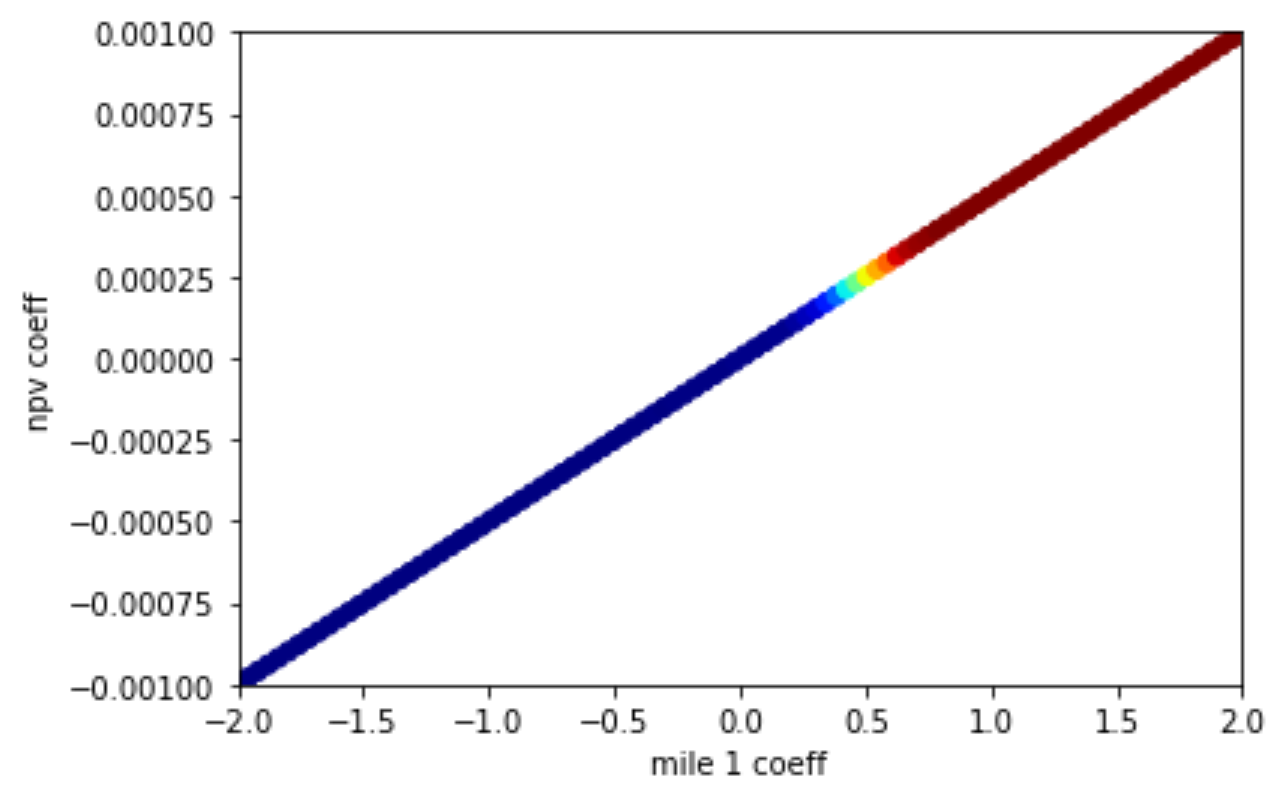
\includegraphics[height=3cm,width=4cm]{AAMAS20Template-submission/figures/rapp100diagmean.png}
    \caption{Diagonal Mean <ADD MORE>}
    \label{fig:diagRappMean}
\end{figure}

\begin{figure}
    \centering
    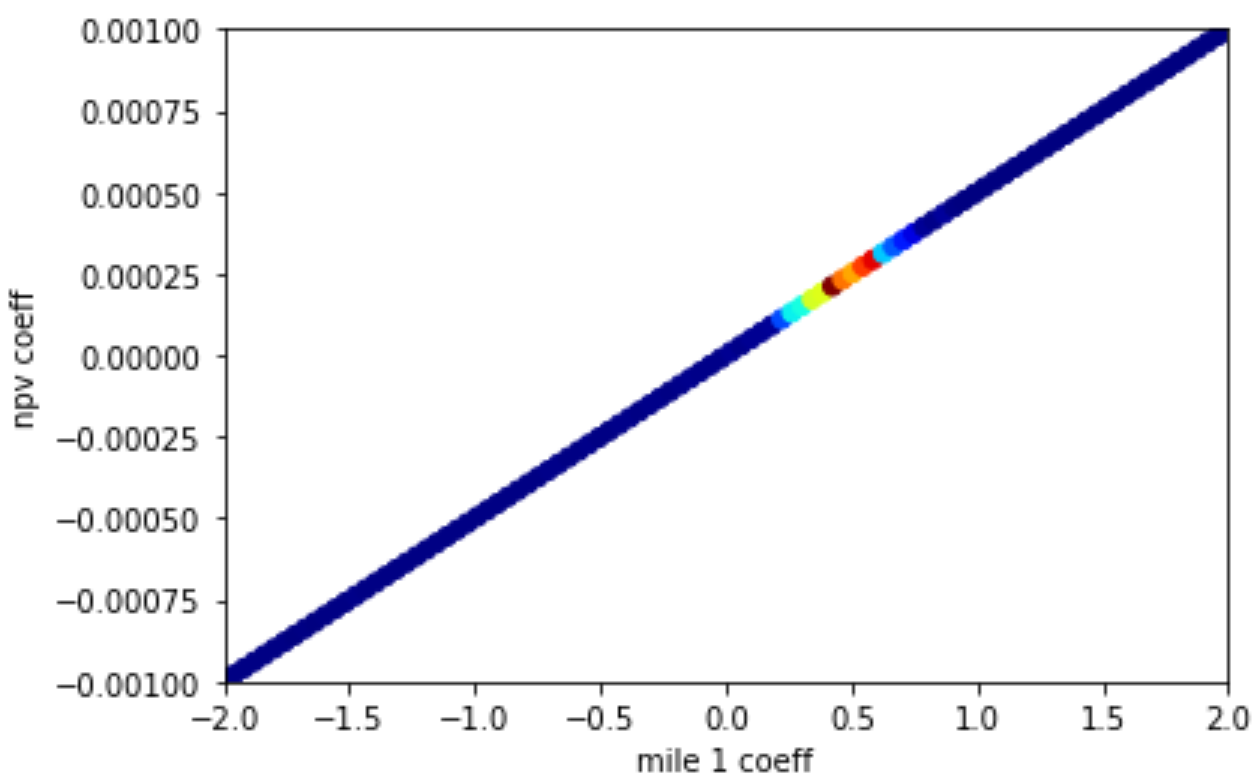
\includegraphics[height=3cm,width=4cm]{AAMAS20Template-submission/figures/rapp100diagstdev.png}
    \caption{Diagonal Stdev <ADD MORE>}
    \label{fig:diagRappStdev}
\end{figure}
\end{comment}

Once the thresholds are set, we conduct three sets of experiments:\\
1. Model \ref{virginia_model} for Rappahannock county\\
2. Model \ref{virginia_model} for SVR region\\
3. Model \ref{san-diego-model} for a zipcode in San Diego\\
First, the search space is initialized with the seed set generation. Classifier is trained on this initial labeled data.
In successive rounds of learning, every time a boundary point is found by binary search, a fixed number of points are queried and labeled in the neighborhood of the boundary point. These labeled points are used to train the classifier in every round.

In order to initiate a binary search that leads to meaningful generation of boundary point, two types of approaches are tried for each set of experiments. These approaches are used to find a start point for binary search. The first set of endpoints is chosen to be the diagonal of the parameter search space. From the next round, points are chosen intelligently by exploiting the knowledge of $boundaryPoints$ and $evaluatedPoints$.\\
First Approach:
Use SVM linear classifier and generate points near/on the SVM linear boundary.
Choose one point from this set that is far away from existing points in $evaluatedPoints$ and $boundaryPoints$.\\
Second approach:
Train Random Forest classifier with $evaluatedPoints$. Then, query points in the search space such that their neighbors collectively have roughly equal distribution pf labels indicating that they are close to the boundary. Choose one point from this set that is far away from existing points in $evaluatedPoints$ and $boundaryPoints$.\\

